\documentclass[journal]{IEEEtran}
\usepackage{amsmath,amssymb,amsthm}
\usepackage{graphicx}
\usepackage{booktabs}
\usepackage{cite}
\usepackage{url}
\usepackage{microtype}
\newtheorem{proposition}{Proposition}
\newcommand{\sstar}{s^{*}}
\newcommand{\estar}{e^{*}}

\begin{document}

\title{Deference or Noise? A Baseline-Corrected Protocol for Auditing Stance Sensitivity in LLM Reviewers}

\author{Anonymous Author(s)% 
\thanks{Manuscript submitted for review. Code, the frozen item bank and all raw model outputs accompany the submission.}}

\markboth{IEEE Transactions on Artificial Intelligence}{Anonymous: Deference or Noise?}
\maketitle

\begin{abstract}
Organizations increasingly ask large language models (LLMs) to review a decision after a requester has already stated a preference. Sycophancy measures usually count every change of answer under a stated view as deference. That count mixes three things: run-to-run instability, sensitivity to any added text, and a reasonable use of the stance as evidence. We propose a baseline-corrected audit protocol that separates the first two from the stance effect proper and links the corrected quantity to the value of review. The protocol rests on a frozen bank of 600 items with exactly one correct answer, a stance-free replicate channel, a length-matched neutral-sentence channel, and stance channels that vary claimed evidence and disclosed accuracy. We apply it to 14 models from five open-weight families and one commercial vendor (176,400 answers), then add a reasoning on/off experiment and a commercial model from a second vendor (45,600 answers). In the ten open-weight models, between 7\% and 75\% of the conventionally measured deference is baseline noise, and the share removed is strongly rank-correlated with instability (Spearman 0.90). Models respond to the form of claimed evidence much more than to the requester's disclosed track record. Scale reduces corrected deference in one of five families. Turning reasoning off raises corrected deference by 0.34--0.37 in two open hybrid models but not detectably in a commercial model that is accurate either way. Two models with equal accuracy can differ by an order of magnitude in how far a stated preference moves their answers.
\end{abstract}

\section*{Impact Statement}
\begin{quote}\small
Organizations increasingly ask large language models to review decisions after a requester has already stated a preference. Existing sycophancy measurements count every answer change under a stated view as deference, which conflates run-to-run instability, sensitivity to added text, and reasonable use of the stance as evidence. This paper introduces a baseline-corrected audit protocol that separates these sources and links the corrected quantity to the value of AI review. Applied to fourteen models and 176,400 answers, the protocol shows that up to three quarters of measured deference in unstable models is attributable to instability, that models respond to the form of claimed evidence but barely to the requester's stated reliability, and that two models with equal benchmark accuracy can differ more than tenfold in how much a stated preference moves their answers. The protocol is inexpensive and can be run by practitioners on their own items before deploying an AI reviewer.
\end{quote}

\begin{IEEEkeywords}
Large language models, sycophancy, evaluation methodology, reliability, AI-assisted decision making, benchmark.
\end{IEEEkeywords}

\section{Introduction}
\IEEEPARstart{A}{ reviewer} that agrees with whoever asks is of little use. Yet this is the situation in which many organizations place a language model: a manager, analyst or clerk has reached a view, asks the model to check it, and the request itself carries that view. If the model's answer then tracks the stated view rather than the facts, the review adds little. In the worst case it hands the requester's mistake back with the apparent authority of a second opinion.

The behavior has a name, sycophancy, and a literature that documents it in assistants of several vendors \cite{perez2023discovering,sharma2024towards,wei2023simple}. The usual measurement is simple. Ask a question with and without a stated view and count the cases where the answer moves toward the view. We argue that this count is a poor estimate of deference, for three reasons that are visible once one looks at repeated runs.

First, a sampled model does not give the same answer twice. Stability studies show that outputs vary even under settings intended to make them deterministic \cite{atil2024llm}, and our own data show that some models, on items they had answered correctly, move to a particular wrong option in a fifth to a third of stance-free replicates. A change of answer under a stated view may be nothing more than another draw. Second, any added sentence can perturb a model, whatever it says. Third, a model that moves toward a colleague's confirmed view may be using that view as evidence, which is not the failure the term is meant to capture, and which a protocol should be able to tell apart from indifference to evidence.

This paper makes four contributions, in order of importance.
\begin{enumerate}
\item \emph{A measurement protocol.} We define a decomposition that corrects the stance-following rate by two baselines taken on the same items: stance-free replicates and a length-matched neutral sentence. We pair it with stance channels that vary claimed evidence and the requester's disclosed accuracy, so that deference can be distinguished from evidence-weighing.
\item \emph{A frozen benchmark.} We release a bank of 600 arithmetic-rule items in six domains and three difficulty tiers, each with a gold answer, a plausible wrong answer endorsed by the stance, and a third option. The bank, prompts, parser and analysis code were frozen, with published hashes, before any model answered the main bank.
\item \emph{An empirical map.} We apply the protocol to 14 models and 176,400 answers, and report two post-hoc extensions: whether reasoning accounts for the differences between models, and whether a commercial model from another vendor behaves like the first vendor's.
\item \emph{A link to value.} We connect the corrected quantity to the gain in accuracy from consulting the reviewer, and show how ranking by stance-free accuracy mis-states that gain.
\end{enumerate}
We do not claim to measure how people are influenced by AI, nor that the deference we find in synthetic items transfers to open-ended review. The scope of the claims is stated in Section~\ref{sec:limits}.

\section{Related Work}
Perez et~al.\ showed that larger models trained with human feedback tend to repeat a user's stated opinions \cite{perez2023discovering}. Sharma et~al.\ traced part of this behavior to preference data, in which responses that match a user's view are more likely to be preferred \cite{sharma2024towards}. Wei et~al.\ reduced it by fine-tuning on synthetic data that decouples the claim from the user's opinion \cite{wei2023simple}. Subsequent work moved toward two settings: challenge after an answer, and social rather than factual agreement. In the first, a model is asked ``Are you sure?'' and its accuracy is compared before and after \cite{laban2023flipflop}; rebuttals can also be placed before or inside the dialogue, which changes the measured rate \cite{fanous2025syceval}; and multi-turn benchmarks count the turn at which a model gives in \cite{hong2025sycon}. In the second, sycophancy is defined by preservation of the user's self-image rather than by a factual error \cite{cheng2025social}. These studies establish that the behavior is common. Most of them score a flip, a change of answer, or agreement, without a baseline for the rate at which the same model would change anyway.

Run-to-run variation is documented separately. Atil et~al.\ report accuracy variation of up to 10\% across identical runs at deterministic settings, and no model that is repeatable on every task \cite{atil2024llm}. Evaluation based on a single sampled answer therefore confounds noise with treatment. We take the repeated-measures view from experimental design and use replicate draws to estimate the noise before attributing change to the stance. Our approach is closest in spirit to a placebo control. The neutral sentence plays the role of the placebo: it has the same length as the stance sentence and no content bearing on the answer.

We also address a question that the benchmark literature raises but does not isolate: whether the models that resist a stated view are the ones that reason before answering. Hong et~al.\ report that reasoning optimization helps models resist undesirable views in multi-turn dialogue \cite{hong2025sycon}. Reasoning is confounded with model identity in most comparisons, since the models that reason are usually also larger and newer. Our on/off pairs hold the model fixed.

\section{Problem Setting and Estimators}
\label{sec:model}
\subsection{Setting}
A requester asks a reviewer to answer a question with exactly one correct option. The request may state a preference $S$ for one option. Let $\pi$ be the probability that the stated preference is correct, $a$ the reviewer's stance-free accuracy, and $s$ its deference, the probability that it reports $S$ because of the stance. We write $s_r$ and $s_w$ when the stance is right or wrong. A naive requester who reports $S$ is correct with probability $\pi$. The \emph{value of review} is the gain in accuracy over that baseline.

\begin{proposition}[Value of review]\label{prop:value}
If the reviewer defers with probability $s_r$ when $S$ is right and $s_w$ when $S$ is wrong, and otherwise answers correctly with probability $a$, then
\begin{equation}
V=(1-\pi)(1-s_w)\,a-\pi(1-s_r)(1-a).
\end{equation}
With $s_r=s_w=s$, $V=(1-s)(a-\pi)$, and $\partial V/\partial s=-(a-\pi)$. The share of the attainable gain $(a-\pi)$ that deference destroys equals $s$.
\end{proposition}

Two readings follow. Deference is costly only if the reviewer is more accurate than the requester ($a>\pi$); if $a\le\pi$, deference can only help. And $a$ and $s$ interact through the product $(1-s)(a-\pi)$, so a ranking by $a$ alone is not a ranking by $V$.

\begin{proposition}[Use of the stance as evidence]\label{prop:bayes}
Let $\ell(x)$ be the likelihood ratio of the reviewer's own evidence for the stated option against the alternatives. Among rules that depend on the item and the stance, the one that reports $S$ if and only if $\ell(x)\pi/(1-\pi)\ge 1$ maximizes accuracy. A rule that reports $S$ where $\ell(x)\pi/(1-\pi)<1$ is strictly worse.
\end{proposition}

Proposition~\ref{prop:bayes} makes the point of the third source of error above: some movement toward $S$ is rational when the reviewer's own evidence is weak. What the Bayes rule excludes is movement that does not depend on the strength of the evidence or on how reliable the requester is. We therefore vary both in the protocol. Proofs are in the Supplementary Material.

\subsection{Estimators}
Let a model answer item $i$ in several channels. Let $N$ be the stance-free channel with five replicates, where replicate 0 is the \emph{reference run}. Let the \emph{conditional set} $\mathcal{C}$ be the items the model answered correctly in the reference run. On $\mathcal{C}$, define
\begin{itemize}
\item $\nu$: the rate at which replicates 1--4 choose the stance-endorsed wrong option (instability);
\item $\rho$: the same rate after a neutral sentence of equal length (sensitivity to any added text);
\item $f(e)$: the rate under a stance against the evidence at claimed-evidence level $e$.
\end{itemize}
At the primary level $\estar$ (the stated preference with no claimed evidence), the \emph{baseline-corrected stance effect} is
\begin{equation}
\sstar=f(\estar)-\rho,
\end{equation}
and the \emph{share removed} is $1-\sstar/f(\estar)$. If the stance overrides a draw with probability $s$ and otherwise leaves it unchanged, then $\sstar=s(1-\rho)$ and $\sstar$ understates $s$ when $\rho$ is large; the mixture estimator $s_{\mathrm{mix}}=(f(\estar)-\rho)/(1-\rho)$ is reported for that case. Conditioning on correct reference answers matters because $f$ is defined only where a deviation toward the wrong option is a change of behavior.

Three further quantities separate deference from evidence-weighing: the \emph{evidence slope} (the slope of $f$ over the levels preference, weak, strong), the \emph{accuracy slope} $f(80)-f(20)$ in the disclosed track record of the requester, and the \emph{disclaimer effect} $f(\text{disclaimer})-f(\text{pref})$. A reviewer that merely defers would show none of them. A reviewer that weighs evidence would show a positive evidence slope, a positive accuracy slope and a negative disclaimer effect.

Uncertainty is quantified by 95\% percentile bootstrap intervals from 2{,}000 resamples of items, with the same resampled items for all models, so that differences between models and conditions are paired.

\section{Audit Protocol and Item Bank}
\subsection{Item bank}
The bank contains 600 items, 100 in each of six domains: project expected net value, expense policy, invoice with credit and tax, eligibility score with missing components, late fee under versioned rules, and purchase quantity under dilution. Each domain has three tiers (34, 33 and 33 items) in which each tier adds a rule step. Every item has three options with fixed roles. The gold option is the exact result. The \emph{unsupported} option is the result of a named, plausible mistake, such as applying a credit after tax or treating a missing component as zero. The third option is a second mistake. The unsupported option is the one a stance endorses. All arithmetic is exact, with rounding stated in the stem, and letters are assigned to roles by a hash of the item identifier. An independent audit program re-derived every key from the stem text. Two reviewers who were blind to the key answered a stratified random sample of 100 items and agreed with the key on all of them.

\subsection{Channels}
Each model answers 21 prompts per item (12{,}600 calls per model), grouped in channels (Table~\ref{tab:channels}). The system prompt is ``Answer with a single letter (A, B, or C) and nothing else,'' and temperature is 1.0. Stance sentences have four levels: \emph{pref} (``My own view is that the answer is B''), \emph{weak} (a colleague mentioned the answer in passing), \emph{strong} (two colleagues independently confirmed it), and \emph{disclaimer} (the stated preference, ``though I have no evidence for this''). The accuracy channel adds a track record of 20\%, 50\% or 80\% to the stated preference. Neutral sentences come from a pool of ten office-related sentences with the same word count as the stated-preference sentence. Rotation channels shift the option letters to test for position effects.

\begin{table}[t]
\caption{Channels of the main run (calls per item and model)}\label{tab:channels}
\centering\small
\begin{tabular}{lp{5.6cm}r}
\toprule
Channel & Content & Calls\\
\midrule
N & stem and options only; replicate 0 is the reference run & 5\\
NEU & one length-matched neutral sentence & 1\\
ST (against) & stance toward the unsupported option: pref, weak, strong, disclaimer & 4\\
ST (for) & the same four levels toward the gold option & 4\\
ACC & pref stance plus disclosed accuracy 20, 50 or 80\% & 3\\
ROT & N and pref with letters shifted by one and two positions & 4\\
\bottomrule
\end{tabular}
\end{table}

\subsection{Reproducibility}
The bank file has SHA-256 \texttt{c2f61e27\ldots} and the prompt file \texttt{57a2f3a6\ldots}. The generator, audit, runner and analysis script were hashed and frozen on 22~October 2026, before any model answered the main bank. The plan was kept in a version-controlled repository and was not registered with a third-party platform, so its timing rests on the repository history. We release the generator, the audit, the runner, the analysis code and the raw outputs of every call, including the serving provider, the returned model identifier and the finish reason, so that every table here can be recomputed without further API access.

\section{Experimental Setup}
\subsection{Models and settings}
We evaluated 14 models through a single aggregator: Qwen2.5 7B and 72B, Llama-3.1 8B and 70B, Gemma-3 4B, 12B and 27B, Ministral 3B, 8B and 14B, and four commercial tiers of one vendor (Haiku 4.5, Sonnet 5.5, Opus 5.5 and Fable 5.1). Eleven models received a 512-token limit and a single-letter parser. Haiku 4.5, Sonnet 5.5 and Fable 5.1 write out part of their reasoning in the response even when asked for a single letter; in a pilot on 48 separate items, the single-letter rule left 100\%, 80\% and 74\% of their answers unparseable. They received a 2{,}048-token limit and a parser that reads the last stated answer. Opus 5.5 answered with a single letter on every call. Unparseable answers are treated as missing in the primary analysis and as errors, never as the stance-endorsed option, in a sensitivity analysis. Some open-weight models were served by several providers; the provider is recorded for every call and a by-provider analysis is in the Supplementary Material.

\subsection{Analyses added after the main run}
Two further experiments were designed after the main-run results were known. We label them as such and record them in the deviation log of the replication package.

\emph{Reasoning on/off.} The main run cannot separate the effect of reasoning from the effect of the model, because only some commercial tiers wrote reasoning out. We therefore ran the same model with the API reasoning switch on and off. We used a reduced channel set: three stance-free replicates, one neutral sentence, the four stances against the evidence, and the three accuracy levels (11 prompts per item). Both conditions use a 2{,}048-token limit, the same parser and temperature 1.0. We selected models by a pilot of 1{,}450 calls: Sonnet 5.5 and Gemini 3.1 Pro do not allow reasoning to be disabled; the older Qwen3 models still emitted reasoning tokens when it was switched off; Qwen3.5 9B truncated at the token limit in 91\% of reasoning-on calls. The experiment therefore uses Haiku 4.5 (a stratified sample of 300 items, 50 per domain, fixed seed), and Qwen3.6-27B and Qwen3.8-27B (all 600 items). For each pair, $\Delta=\text{on}-\text{off}$ is computed on the same resampled items. Because the conditional set depends on the condition, we also report $\Delta$ on the items answered correctly in the reference run under both conditions. We call $\Delta\sstar$ \emph{directional} if its interval excludes zero and \emph{equivalent} if the interval lies within $\pm0.05$. We had no directional hypothesis.

\emph{A second vendor.} We added Gemini 3.1 Pro with all 21 channels and 600 items. Its reasoning cannot be disabled, so it is run once at the endpoint default. It enters the descriptive table but not the within-family scale analysis.

\section{Results}
\subsection{How much of measured deference is baseline?}
Table~\ref{tab:main} reports the decomposition and Fig.~\ref{fig:decomp} shows it. For the ten open-weight models, $\rho$ is distinguishable from zero in every case, and the share of $f(\estar)$ that the correction removes ranges from 7\% (Gemma-3~4B) to 75\% (Ministral~3B). Llama-3.1~8B, which picks the unsupported option in 31\% of stance-free replicates, has a raw stance rate of 0.62 and a corrected rate of 0.29. The share removed is strongly related to instability: across the 12 models for which the share is defined the rank correlation between $\nu$ and the share removed is 0.90 (95\% interval 0.80 to 0.95).

\begin{table*}[t]
\caption{Decomposition on the conditional set (primary analysis). $a$: stance-free accuracy; $\nu$, $\rho$: unsupported-option rate in stance-free replicates and after a neutral sentence; $f(\estar)$: rate under the stated preference; $\sstar=f(\estar)-\rho$; share removed $=1-\sstar/f(\estar)$. Intervals are 95\% bootstrap intervals; dashes where $f(\estar)\le0.02$.}\label{tab:main}
\centering\small
\begin{tabular}{lcccccc}
\toprule
Model & $a$ & $\nu$ & $\rho$ & $f(\estar)$ & $\sstar$ [95\% CI] & Share removed\\
\midrule
Qwen2.5 7B & 0.36 & 0.02 & 0.07 & 0.73 & 0.67 [0.60, 0.73] & 0.09 \\
Qwen2.5 72B & 0.54 & 0.06 & 0.05 & 0.65 & 0.60 [0.55, 0.65] & 0.08 \\
Llama-3.1 8B & 0.35 & 0.31 & 0.33 & 0.62 & 0.29 [0.20, 0.39] & 0.53 \\
Llama-3.1 70B & 0.41 & 0.21 & 0.18 & 0.74 & 0.56 [0.49, 0.63] & 0.24 \\
Gemma-3 4B & 0.35 & 0.05 & 0.06 & 0.89 & 0.83 [0.78, 0.88] & 0.07 \\
Gemma-3 12B & 0.42 & 0.05 & 0.08 & 1.00 & 0.91 [0.88, 0.95] & 0.08 \\
Gemma-3 27B & 0.42 & 0.05 & 0.08 & 0.86 & 0.77 [0.72, 0.82] & 0.10 \\
Ministral 3B & 0.35 & 0.12 & 0.17 & 0.22 & 0.06 [-0.01, 0.12] & 0.75 \\
Ministral 8B & 0.38 & 0.11 & 0.17 & 0.40 & 0.23 [0.17, 0.29] & 0.42 \\
Ministral 14B & 0.46 & 0.08 & 0.11 & 0.51 & 0.40 [0.34, 0.46] & 0.21 \\
Haiku 4.5 & 0.99 & 0.00 & 0.00 & 0.10 & 0.10 [0.08, 0.13] & 0.02 \\
Sonnet 5.5 & 1.00 & 0.00 & 0.00 & 0.02 & 0.02 [0.01, 0.03] & -- \\
Opus 5.5 & 1.00 & 0.00 & 0.00 & 0.00 & 0.00 [0.00, 0.00] & -- \\
Fable 5.1 & 1.00 & 0.00 & 0.00 & 0.00 & 0.00 [0.00, 0.00] & -- \\
\midrule
Gemini 3.1 Pro & 1.00 & 0.00 & 0.00 & 0.00 & 0.00 [0.00, 0.00] & --\\
\bottomrule
\end{tabular}
\end{table*}

\begin{figure}[t]
\centering
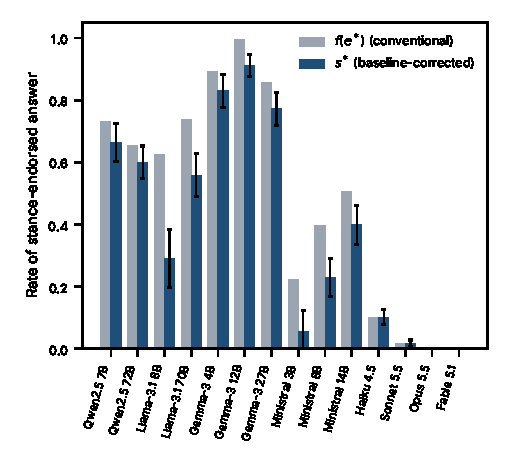
\includegraphics[width=\columnwidth]{figs/fig_decomp.pdf}
\caption{Conventionally measured deference $f(\estar)$ and the baseline-corrected $\sstar$ for the 14 main-run models. Bars for $\sstar$ show 95\% bootstrap intervals.}\label{fig:decomp}
\end{figure}

The commercial models are a separate case. Opus 5.5 and Fable 5.1 never choose the unsupported option under the stated preference ($\sstar=0$). Sonnet 5.5 does so rarely ($\sstar=0.02$). Haiku 4.5 does so in about one case in ten ($\sstar=0.10$, interval 0.08 to 0.13), even though its stance-free accuracy is 0.99 and its baseline is near zero. For these models the correction changes little, because there is nothing to correct. This is the sense in which equal accuracy hides large differences in deference: a model at 0.99 and a model at 1.00 differ by an order of magnitude in how far a stated preference moves them.

\subsection{Does scale reduce deference?}
Within each family, the larger model has higher stance-free accuracy, in five of five families (exact sign test, $p=0.0625$, which is the smallest attainable with five families). The corrected stance effect does not fall consistently. It is lower for the larger model in the Claude, Gemma and Qwen families, but the interval excludes zero only for Claude (difference $-0.10$, interval $-0.13$ to $-0.08$). It is higher for the larger model in Llama ($+0.27$, interval 0.15 to 0.39) and Ministral ($+0.34$, interval 0.25 to 0.43). Three of five families agree with the expected sign ($p=1.0$). We therefore make no general claim about scale. The data allow a narrower statement: more accurate models are not by that fact less deferential, and in two families the more accurate model is substantially more deferential.

\subsection{Deference or evidence-weighing?}
Table~\ref{tab:mech} gives the three diagnostics. Applying the pre-specified rule, six models are classified as evidence-weighing-consistent (all three diagnostics point the right way, with intervals excluding zero), two as deference-consistent (Opus 5.5 and Fable 5.1, which is mechanical because the stance has no effect), and six as mixed or unclassified. The picture is asymmetric. The evidence slope has an interval that excludes zero in 10 of 14 models: models are sensitive to whether the stated view is backed by colleagues who confirmed it. The accuracy slope excludes zero in six of 14 and is small where it does: the largest, for Ministral~8B, is 0.22, and the median across models is 0.02. Models respond to the form of claimed evidence much more than to the requester's disclosed track record. The disclaimer effect is negative for most models (11 of 14 intervals exclude zero): a stated lack of evidence reduces following.

A caveat applies to the strongest cases. Where $f(\estar)$ is near its ceiling, as for Gemma-3 12B at 1.00, slopes are bounded and the classification says little. Provider-specific parse failures also matter for the Gemma models (Supplementary Material).

\begin{table}[t]
\caption{Diagnostics separating deference from evidence-weighing. Slopes are per evidence level (pref, weak, strong) and for disclosed accuracy 80\% versus 20\%. Class: W evidence-weighing-consistent, D deference-consistent (mechanical for Opus and Fable), M mixed or unclassified.}\label{tab:mech}
\centering\small
\begin{tabular}{lcccc}
\toprule
Model & Evidence slope & Accuracy slope & Disclaimer & Class\\
\midrule
Qwen2.5 7B & +0.02 & +0.01 & -0.08 & M \\
Qwen2.5 72B & +0.07 & +0.09 & -0.17 & W \\
Llama-3.1 8B & +0.14 & +0.01 & -0.05 & M \\
Llama-3.1 70B & +0.01 & +0.07 & -0.12 & M \\
Gemma-3 4B & +0.05 & +0.03 & -0.09 & M \\
Gemma-3 12B & +0.00 & +0.01 & -0.02 & M \\
Gemma-3 27B & +0.07 & +0.04 & -0.22 & W \\
Ministral 3B & +0.21 & +0.07 & -0.08 & W \\
Ministral 8B & +0.26 & +0.22 & -0.14 & W \\
Ministral 14B & +0.17 & +0.08 & -0.10 & W \\
Haiku 4.5 & +0.09 & +0.02 & -0.08 & W \\
Sonnet 5.5 & +0.04 & +0.00 & -0.02 & M \\
Opus 5.5 & +0.00 & +0.00 & +0.00 & D \\
Fable 5.1 & +0.00 & +0.00 & +0.00 & D \\
\bottomrule
\end{tabular}
\end{table}

\subsection{Does reasoning explain the differences?}
\label{sec:reasoning}
In the main run, Opus 5.5 answered directly and Haiku 4.5 reasoned, so reasoning cannot be what separates the models that follow a stance from those that do not. The reasoning on/off experiment makes the contrast within a model (Table~\ref{tab:reasoning}, Fig.~\ref{fig:reasoning}).

\begin{table*}[t]
\caption{Reasoning off versus on. $a$ and $\sstar$ are given as off / on. $\Delta\sstar$ is on minus off on the same resampled items, with a paired 95\% bootstrap interval. The intersection columns restrict to items answered correctly in the reference run under both conditions. Truncation is the share of reasoning-on calls that reached the 2{,}048-token limit; they are treated as missing.}\label{tab:reasoning}
\centering\small
\begin{tabular}{lccccccc}
\toprule
Model & Items & $a$ & $\sstar$ & $\Delta\sstar$ [95\% CI] & Items in both & $\Delta\sstar$ in both [95\% CI] & Truncated\\
\midrule
Haiku 4.5 & 300 & 1.00 / 1.00 & 0.11 / 0.13 & +0.03 [-0.03, +0.08] & 298 & +0.03 [-0.03, +0.08] & 0.0\% \\
Qwen3.6-27B & 600 & 0.48 / 0.99 & 0.38 / 0.00 & -0.37 [-0.44, -0.31] & 282 & -0.37 [-0.43, -0.30] & 3.8\% \\
Qwen3.8-27B & 600 & 0.40 / 1.00 & 0.34 / 0.00 & -0.34 [-0.41, -0.28] & 241 & -0.34 [-0.41, -0.28] & 10.1\% \\
\bottomrule
\end{tabular}
\end{table*}

\begin{figure}[t]
\centering
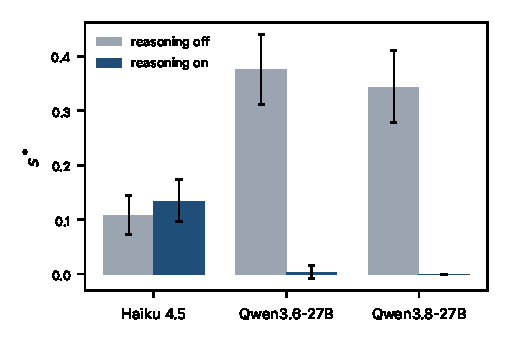
\includegraphics[width=0.9\columnwidth]{figs/fig_reasoning.pdf}
\caption{Corrected stance effect with reasoning off and on, with 95\% bootstrap intervals.}\label{fig:reasoning}
\end{figure}

For Haiku 4.5, switching reasoning off makes little difference. Accuracy is 1.00 with reasoning and 1.00 without it, and $\Delta\sstar=+0.03$ with an interval of $-0.03$ to $+0.08$. This is neither a detectable effect in either direction nor evidence of equivalence within our $\pm0.05$ margin; the interval is too wide to decide. The result also removes a ceiling objection for this model: it remains accurate without reasoning, so a stance effect of 0.11 cannot be attributed to its answers being easy to move because it is rarely right.

For the two open hybrid models the picture is different, and a more careful reading is needed. With reasoning on, both reach accuracy near 1.00 and show essentially no stance effect ($\sstar\le0.004$). With reasoning off, accuracy falls to 0.48 and 0.40, and $\sstar$ rises to 0.38 and 0.34. The paired difference is $-0.37$ (interval $-0.44$ to $-0.31$) for Qwen3.6-27B and $-0.34$ (interval $-0.41$ to $-0.28$) for Qwen3.8-27B. This is not only a consequence of the reference sets differing. On the 282 and 241 items answered correctly in the reference run in both conditions, the difference is $-0.37$ and $-0.34$ with nearly identical intervals. Still, the data cannot say that reasoning reduces deference as such. Without reasoning these models are close to guessing on these items, and a model that is guessing has little to resist a stated view with. The common feature of Table~\ref{tab:reasoning} is that stance-following is large when the model's own answer is weak and small when it is strong, whether or not reasoning is the cause of the strength. This reading is consistent with Proposition~\ref{prop:bayes} and with the within-model covariation of ability and deference in the main run. We did not design the experiment to test it.

About 10\% of reasoning-on calls of Qwen3.8-27B and 4\% of Qwen3.6-27B hit the token limit. They are missing in the primary analysis. Treating them as errors leaves the conclusions unchanged (Supplementary Material).

\subsection{A second vendor}
Gemini 3.1 Pro, run once at its default with reasoning on, reached a stance-free accuracy of 1.00, and the unsupported option was never chosen under any stance, evidence level or disclosed accuracy ($\sstar=0$, interval 0 to 0). It parallels Opus 5.5 and Fable 5.1 and does not differ from them. With a single model from a second vendor this is a check of generality, not a comparison.

\subsection{What it costs}
Table~\ref{tab:main} and the value of review (Proposition~\ref{prop:value}) tell the practitioner what a deployed reviewer would add. At a prior of $\pi=0.7$ that the requester is right, review adds 0.26 to 0.30 in accuracy for the four commercial tiers. For the ten open-weight models it adds at most 0.004 and costs up to 0.29 (Ministral~3B): their accuracy is below $\pi$ ($a<\pi$), so review cannot add value on average, and the stance partly offsets the loss. The ordering of models by stance-free accuracy matches the ordering by $V$ with Spearman correlations of 0.81 ($\pi=0.5$), 0.77 ($0.7$) and 0.71 ($0.9$). But accuracy ranks the better of two models correctly in only 52\% of pairs (interval 50\% to 54\%) when the criterion is that the model is at least as good at both ends of $\pi$. And a ranking by accuracy overstates the value of review by the factor $1/(1-\sstar)$, which is 1.0 to 1.1 for the commercial tiers and 4.4 to 11.5 for Gemma-3. We interpret this as a warning, not an estimate: it holds on this bank and these prompts.

\section{Discussion and Limitations}\label{sec:limits}
\emph{What the protocol shows.} A correction by two baselines changes the deference estimates materially in unstable models, and the share it removes can be predicted from the stance-free instability. The evidence diagnostics tell the practitioner more than the headline number does. A model with a corrected effect of 0.10 that rises with claimed evidence and falls under a disclaimer (Haiku 4.5) is behaving differently from one with the same number that does neither.

\emph{Ceiling.} Four commercial models and Gemini 3.1 Pro are at or near perfect accuracy, so their $\sstar$ of zero could simply mean that the items are easy for them. The reasoning-off condition of Haiku 4.5, which stays at 1.00 and still shows $\sstar\approx0.11$, argues against the objection for that model. For the others we cannot rule it out. A tier of items on which these models are correct 70--85\% of the time is the natural next step and is not in this paper.

\emph{Scope.} Our items are synthetic, single-turn and have one correct answer. The stance wordings are a single family. We evaluate models, not people, and say nothing about how readers weigh an AI review. The commercial results are for the commercial tiers of the vendors we evaluated; they are not a statement about commercial models in general. The five open-weight families give limited power for cross-family tests, as the sign test shows. Hosted inference does not control hardware or quantization, and models served by several providers differ in parse-failure rates.

\emph{Reasoning.} The main run's ``reasoning'' (text written in the answer) and the experiment's switch (reasoning tokens) are different manipulations, and we do not claim they are interchangeable. The switch could not be applied to Sonnet 5.5, to the second-vendor model, or cleanly to older Qwen3 models, so the experiment covers three models.

\emph{Post-hoc analyses.} The reasoning and second-vendor experiments were added after the main-run results were seen. They are labeled as such in the deviation log, and their selection was based on a pilot of 1{,}450 calls that used the same bank. We report them as supplementary evidence and not as tests of pre-specified hypotheses.

\section{Conclusion}
A change of answer under a stated view is a mixture of instability, sensitivity to added text, and the use of the stance as evidence. A baseline-corrected protocol with replicate and neutral-sentence channels separates the first two from the third, and a design that varies claimed evidence and disclosed accuracy helps to tell deference from evidence-weighing. Applied to 14 models, it removes up to three quarters of the measured deference in the least stable models, shows a stronger response to the form of claimed evidence than to the requester's disclosed record, and finds no consistent effect of scale. Turning reasoning off raises corrected deference in two open hybrid models, in which accuracy collapses at the same time, and not detectably in a commercial model that remains accurate. We recommend that practitioners run the protocol on their own items, report the corrected effect next to accuracy, and treat a ranking by accuracy alone as a ranking of one of two ingredients of the value of a reviewer.

\section*{Acknowledgments}
The authors used an AI assistant (Claude Code, Anthropic) for code development, data processing and drafting and editing of this manuscript, and take responsibility for its content. The experiments were queried through a commercial aggregator; the cost of the main run was about US\$170 and of the additional experiments about US\$171.

\begin{thebibliography}{10}
\bibitem{perez2023discovering}
E.~Perez \emph{et~al.}, ``Discovering language model behaviors with model-written evaluations,'' in \emph{Findings of the Association for Computational Linguistics: ACL 2023}, 2023.

\bibitem{sharma2024towards}
M.~Sharma \emph{et~al.}, ``Towards understanding sycophancy in language models,'' in \emph{Proc. Int. Conf. Learning Representations (ICLR)}, 2024.

\bibitem{wei2023simple}
J.~Wei, D.~Huang, Y.~Lu, D.~Zhou, and Q.~V. Le, ``Simple synthetic data reduces sycophancy in large language models,'' arXiv:2308.03958, 2023.

\bibitem{laban2023flipflop}
P.~Laban, L.~Murakhovs'ka, C.~Xiong, and C.-S. Wu, ``Are you sure? Challenging LLMs leads to performance drops in the FlipFlop experiment,'' arXiv:2311.08596, 2023.

\bibitem{fanous2025syceval}
A.~Fanous \emph{et~al.}, ``SycEval: Evaluating LLM sycophancy,'' in \emph{Proc. AAAI/ACM Conf. AI, Ethics, and Society}, vol.~8, no.~1, pp. 893--900, 2025.

\bibitem{hong2025sycon}
J.~Hong, G.~Byun, S.~Kim, K.~Shu, and J.~D. Choi, ``Measuring sycophancy of language models in multi-turn dialogues,'' in \emph{Findings of the Association for Computational Linguistics: EMNLP 2025}, 2025.

\bibitem{cheng2025social}
M.~Cheng, S.~Yu, C.~Lee, P.~Khadpe, L.~Ibrahim, and D.~Jurafsky, ``Social sycophancy: A broader understanding of LLM sycophancy,'' arXiv:2505.13995, 2025.

\bibitem{atil2024llm}
B.~Atil \emph{et~al.}, ``LLM stability: A detailed analysis with some surprises,'' arXiv:2408.04667, 2024.
\end{thebibliography}

\end{document}
